\documentclass[11pt,a4paper]{article}

\usepackage[utf8]{inputenc}
\usepackage[T1]{fontenc}
\usepackage[french]{babel}
\usepackage{lmodern}
\usepackage{microtype}
\usepackage[margin=2.5cm]{geometry}
\usepackage{amsmath,amssymb,amsthm}
\usepackage{graphicx}
\usepackage{booktabs}
\usepackage{caption}
\usepackage{enumitem}
\usepackage[colorlinks=true,linkcolor=blue,citecolor=blue,urlcolor=blue]{hyperref}

\graphicspath{{figures/}}

\newcommand{\E}{\mathbb{E}}
\newcommand{\N}{\mathcal{N}}
\newcommand{\BCR}{\mathrm{BCR}}
\newcommand{\RMSE}{\mathrm{RMSE}}
\newcommand{\EKF}{\mathrm{EKF}}
\DeclareMathOperator{\atantwo}{atan2}
\DeclareMathOperator{\diag}{diag}

\theoremstyle{remark}
\newtheorem*{remarque}{Remarque}

\title{\textbf{Bornes de Cramér-Rao pour le filtrage bayésien\\[2pt]
\large Application au pistage par mesures d'angles}}
\author{Mohamed Benloughmari \and Fatimetou Narjah}
\date{TP3 --- ENSTA, 2026}

\begin{document}

\maketitle

\section*{Introduction}

La borne de Cramér-Rao (BCR) fournit une limite inférieure sur l'erreur quadratique de tout estimateur. Elle permet ainsi d'évaluer la performance d'un estimateur, ou de prédire la performance optimale atteignable pour un problème donné, à partir du seul modèle.
Après le cas d'un paramètre statique, déterministe puis aléatoire, ce TP étend la borne au filtrage bayésien grâce à une formulation récursive en temps.
On l'applique au pistage d'une cible par mesures d'angles. La partie~1 traite d'une dynamique non bruitée et utilise la BCR pour optimiser la manœuvre de l'observateur.
La partie~2 traite d'une dynamique bruitée et compare la BCR aux performances réelles d'un filtre de Kalman étendu (EKF).

% =====================================================================
\section{Partie 1 --- Dynamique non bruitée et optimisation de la manœuvre}
% =====================================================================

\subsection{Question Q0 : information de Fisher pour des bruits additifs gaussiens}

On considère un paramètre déterministe $\theta \in \mathbb{R}^d$ observé à travers $n$ mesures
\begin{equation}
y_i = h_i(\theta) + \epsilon_i, \qquad \epsilon_i \sim \N(0, \sigma_i^2), \qquad i = 1, \dots, n,
\end{equation}
où les bruits $\epsilon_i$ sont supposés indépendants et les fonctions $h_i : \mathbb{R}^d \to \mathbb{R}$ différentiables. On note $\dfrac{\partial h_i}{\partial \theta}(\theta) \in \mathbb{R}^{1\times d}$ la jacobienne (vecteur ligne) de $h_i$. On veut montrer que
\begin{equation}
\boxed{\;
J(\theta) = \sum_{i=1}^{n} \frac{1}{\sigma_i^2}
\left(\frac{\partial h_i}{\partial \theta}(\theta)\right)^{\!\top}
\frac{\partial h_i}{\partial \theta}(\theta).
\;}
\label{eq:q0}
\end{equation}

\paragraph{Log-vraisemblance.}
Par indépendance des bruits, la densité des observations se factorise :
\begin{equation}
p(y_{1:n} \mid \theta) = \prod_{i=1}^{n} \frac{1}{\sqrt{2\pi}\,\sigma_i}
\exp\!\left(-\frac{\big(y_i - h_i(\theta)\big)^2}{2\sigma_i^2}\right),
\end{equation}
d'où
\begin{equation}
\ln p(y_{1:n} \mid \theta) = -\sum_{i=1}^{n} \frac{\big(y_i - h_i(\theta)\big)^2}{2\sigma_i^2} + c,
\end{equation}
où la constante $c$ ne dépend pas de $\theta$.

\paragraph{Score.}
En dérivant par rapport à $\theta$, on obtient le score :
\begin{equation}
\nabla_\theta \ln p(y_{1:n} \mid \theta)
= \sum_{i=1}^{n} \frac{y_i - h_i(\theta)}{\sigma_i^2} \left(\frac{\partial h_i}{\partial \theta}(\theta)\right)^{\!\top}
= \sum_{i=1}^{n} \frac{\epsilon_i}{\sigma_i^2}\, g_i,
\qquad g_i \triangleq \left(\frac{\partial h_i}{\partial \theta}(\theta)\right)^{\!\top} \in \mathbb{R}^d.
\end{equation}
On vérifie au passage que le score est centré, puisque $\E[\epsilon_i] = 0$.

\paragraph{Information de Fisher.}
Par définition, $J(\theta) = \E_{Y\mid\theta}\big[\nabla_\theta \ln p \,(\nabla_\theta \ln p)^\top\big]$. Les vecteurs $g_i$ sont déterministes (ils ne dépendent que de $\theta$), donc
\begin{equation}
J(\theta) = \sum_{i=1}^{n} \sum_{j=1}^{n} \frac{\E[\epsilon_i \epsilon_j]}{\sigma_i^2 \sigma_j^2}\, g_i\, g_j^\top .
\end{equation}
Par indépendance et centrage des bruits, $\E[\epsilon_i \epsilon_j] = \sigma_i^2\, \delta_{ij}$. Seuls les termes $i = j$ subsistent :
\begin{equation}
J(\theta) = \sum_{i=1}^{n} \frac{\sigma_i^2}{\sigma_i^4}\, g_i\, g_i^\top
= \sum_{i=1}^{n} \frac{1}{\sigma_i^2}
\left(\frac{\partial h_i}{\partial \theta}(\theta)\right)^{\!\top}
\frac{\partial h_i}{\partial \theta}(\theta),
\end{equation}
ce qui établit~\eqref{eq:q0}. \hfill$\blacksquare$

\paragraph{Vérification par la hessienne.}
On retrouve le même résultat avec la seconde forme $J(\theta) = -\E\big[\nabla_\theta \nabla_\theta^\top \ln p\big]$. En dérivant le score une seconde fois :
\begin{equation}
-\nabla_\theta \nabla_\theta^\top \ln p(y_{1:n} \mid \theta)
= \sum_{i=1}^{n} \frac{1}{\sigma_i^2} \Big( g_i\, g_i^\top - \epsilon_i\, \nabla_\theta^2 h_i(\theta) \Big).
\end{equation}
Le second terme, qui fait intervenir la courbure de $h_i$, est d'espérance nulle car $\E[\epsilon_i] = 0$. Il reste bien~\eqref{eq:q0}.

\paragraph{Écriture matricielle et interprétation.}
En empilant les jacobiennes dans $H(\theta) \in \mathbb{R}^{n\times d}$, de lignes $\frac{\partial h_i}{\partial \theta}(\theta)$, et en posant $R = \diag(\sigma_1^2, \dots, \sigma_n^2)$, on obtient la forme compacte
\begin{equation}
J(\theta) = H(\theta)^\top R^{-1} H(\theta).
\end{equation}
Plusieurs remarques en découlent :
\begin{itemize}[nosep]
  \item \textbf{Additivité.} Chaque mesure indépendante ajoute sa propre contribution $g_i g_i^\top / \sigma_i^2$, qui est de rang~1. Une mesure précise ($\sigma_i$ petit) ou très sensible au paramètre ($\|g_i\|$ grand) apporte beaucoup d'information.
  \item \textbf{Observabilité.} Si les gradients $g_1, \dots, g_n$ n'engendrent pas $\mathbb{R}^d$, $J(\theta)$ est singulière et la BCR n'est pas définie : certaines directions de $\theta$ ne sont pas identifiables. C'est exactement le cas $\varphi = 0$ étudié en Q1.
  \item \textbf{Cas linéaire.} Si $h(\theta) = A\theta$, alors $J = A^\top R^{-1} A$ ne dépend plus de $\theta$, et l'estimateur des moindres carrés pondérés $\hat\theta = (A^\top R^{-1} A)^{-1} A^\top R^{-1} y$ est non biaisé de covariance $J^{-1}$ : il atteint la borne.
  \item \textbf{Lien avec la suite du TP.} Ce résultat fournit le terme de mesure $\frac{1}{\sigma_k^2} H_k^\top H_k$ des récursions~\eqref{eq:bcr_det} et~\eqref{eq:pcrb}, où $H_k = \frac{\partial h_k}{\partial X_k}(X_k)$ est la jacobienne (ligne) de la mesure angulaire.
\end{itemize}

\subsection{Question Q1a : calcul de la BCR (dynamique linéaire non bruitée)}

L'objectif de cette question est d'implémenter le calcul récursif de la borne de Cramér-Rao dans le cas d'une dynamique linéaire non bruitée et de mesures gaussiennes. On considère une cible dont l'état à l'instant $k$ est
\begin{equation}
X_k = \begin{pmatrix} x_k & y_k & \dot{x}_k & \dot{y}_k \end{pmatrix}^{\top},
\end{equation}
de dynamique linéaire et déterministe
\begin{equation}
X_k = \Phi X_{k-1}, \qquad
\Phi = \begin{pmatrix}
1 & 0 & T & 0\\
0 & 1 & 0 & T\\
0 & 0 & 1 & 0\\
0 & 0 & 0 & 1
\end{pmatrix},
\end{equation}
où $T$ est le pas de temps entre deux mesures. La mesure est un azimut bruité,
\begin{equation}
Y_k = h_k(X_k) + \epsilon_k, \qquad
h_k(X_k) = \atantwo\big(y_k - y_k^o,\; x_k - x_k^o\big), \qquad
\epsilon_k \sim \N(0, \sigma_k^2),
\end{equation}
où $(x_k^o, y_k^o)$ sont les coordonnées de l'observateur.

\paragraph{Récursion.}
La matrice d'information initiale est $J_0 = P_0^{-1}$, où $P_0$ est la covariance initiale de l'état. Pour une dynamique non bruitée, la propagation de l'information et l'ajout de la nouvelle mesure s'écrivent :
\begin{equation}
\boxed{\;
J_k = \Phi^{-\top} J_{k-1} \Phi^{-1} + \frac{1}{\sigma_k^2} H_k^\top H_k,
\qquad \BCR_k = J_k^{-1},
\;}
\label{eq:bcr_det}
\end{equation}
où $H_k = \nabla_{X_k} h_k(X_k)$ est le gradient de la fonction de mesure.

\paragraph{Jacobienne de la mesure.}
En posant $\Delta x_k = x_k - x_k^o$ et $\Delta y_k = y_k - y_k^o$, on obtient :
\begin{equation}
H_k = \begin{pmatrix}
-\dfrac{\Delta y_k}{\Delta x_k^2 + \Delta y_k^2} &
\dfrac{\Delta x_k}{\Delta x_k^2 + \Delta y_k^2} &
0 & 0
\end{pmatrix}.
\end{equation}
Les deux dernières composantes sont nulles, car la mesure angulaire ne dépend pas directement des vitesses de la cible.

\paragraph{Implémentation.}
Le calcul est réalisé dans \texttt{cramer\_rao\_deterministe.py}. La méthode \texttt{predict(F)} propage l'information, $J_k^{\mathrm{pred}} = F^{-\top} J_{k-1} F^{-1}$, et la méthode \texttt{update(H,R)} ajoute l'information de mesure, $J_k = J_k^{\mathrm{pred}} + H^\top R^{-1} H$. La borne est ensuite obtenue par inversion de $J_k$, ce qui permet de suivre l'évolution de la précision théorique au cours du temps.

\paragraph{Cas particulier $\varphi = 0$ sans information a priori.}
Lorsque l'observateur ne manœuvre pas ($\varphi = 0$), il suit une trajectoire rectiligne à vitesse constante. Pour étudier l'observabilité du système sans information a priori, on initialise $J_0 = 0_{4\times4}$, puis on applique la récursion~\eqref{eq:bcr_det}. Les valeurs singulières de la matrice d'information finale sont
\begin{equation}
s(J_n) = \begin{pmatrix} 147{,}4345 & 0{,}06849 & 0{,}005350 & 2{,}37\times10^{-16} \end{pmatrix}^{\top}.
\end{equation}
La dernière valeur singulière étant pratiquement nulle, on obtient
\begin{equation}
\boxed{\;\operatorname{rang}(J_n) = 3 < 4.\;}
\end{equation}
La matrice d'information finale est donc singulière, et $J_n^{-1}$ n'existe pas : la BCR complète n'est pas définie. Cette perte de rang traduit la non-observabilité du système. Lorsque l'observateur suit une trajectoire rectiligne à vitesse constante, plusieurs trajectoires de l'émetteur produisent les mêmes mesures angulaires : il existe une direction de l'espace d'état dans laquelle les mesures n'apportent aucune information. Ce résultat met en évidence l'importance de la manœuvre de l'observateur.

\subsection{Question Q1b : optimisation de l'angle de manœuvre}

On cherche le cap que doit adopter l'observateur après sa manœuvre pour minimiser l'incertitude finale sur la position de la cible. La cible se déplace à vitesse constante, sans bruit de dynamique. L'observateur se déplace initialement selon l'axe $+x$ et change instantanément de cap au milieu de la séquence de mesures. Les paramètres de la simulation sont donnés dans le tableau~\ref{tab:q1_param}.

\begin{table}[ht]
\centering
\caption{Paramètres du scénario de la question Q1b.}
\label{tab:q1_param}
\begin{tabular}{ll}
\toprule
Paramètre & Valeur \\
\midrule
Pas temporel & $T = 1$\,s \\
Nombre de mesures & $N = 100$ \\
Écart-type du bruit angulaire & $\sigma_\theta = 1^\circ$ \\
Vitesse de l'observateur & $V_o = 10$\,m/s \\
Vitesse de la cible & $V_c = 5$\,m/s \\
Cap initial de la cible & $-20^\circ$ \\
Position initiale de la cible & $(2000, 2000)$\,m \\
Covariance initiale & $P_0 = \diag(1000^2, 1000^2, 10^2, 10^2)$ \\
\bottomrule
\end{tabular}
\end{table}

Pour chaque valeur du cap $\varphi$ adopté après la manœuvre, on construit la trajectoire nominale de l'observateur, puis on calcule récursivement la matrice d'information. Le critère à minimiser est la somme des bornes de variance sur les deux coordonnées de position à l'instant final $n$ :
\begin{equation}
\boxed{\;
C(\varphi) = \operatorname{tr}\big(\BCR_n(\varphi)_{1:2,\,1:2}\big) = \BCR_{xx}(\varphi) + \BCR_{yy}(\varphi),
\qquad
\varphi_{\mathrm{opt}} = \arg\min_{\varphi \in [0, 360[} C(\varphi).
\;}
\end{equation}
La racine carrée de ce critère, $\mathrm{RMS}_{2D}(\varphi) = \sqrt{C(\varphi)}$, fournit une mesure globale de l'incertitude de position en mètres.

Le programme \texttt{q1\_manoeuvre.py} réalise cette recherche par balayage d'une grille d'angles, dont le pas est fixé par l'option \texttt{--step-deg}. Une première exécution a été effectuée avec un pas de $0{,}1^\circ$, puis une seconde avec un pas de $0{,}01^\circ$ pour vérifier la stabilité du résultat.

\paragraph{Résultats.}
Avec un pas de $0{,}1^\circ$, on obtient un angle optimal de $115^\circ$, pour un critère minimal de $13\,349{,}589$\,m$^2$. Avec un pas de $0{,}01^\circ$, l'angle optimal est de $114{,}9^\circ$, pour un critère minimal de $13\,349{,}546$\,m$^2$. Les deux résultats étant très proches, l'optimum est numériquement stable. On retient :
\begin{equation}
\boxed{\;
\varphi_{\mathrm{opt}} = 114{,}9^\circ,
\qquad
C_{\min} = 13\,349{,}546\ \text{m}^2,
\qquad
\mathrm{RMS}_{2D,\min} = 115{,}540\ \text{m}.
\;}
\end{equation}

\begin{figure}[ht]
\centering
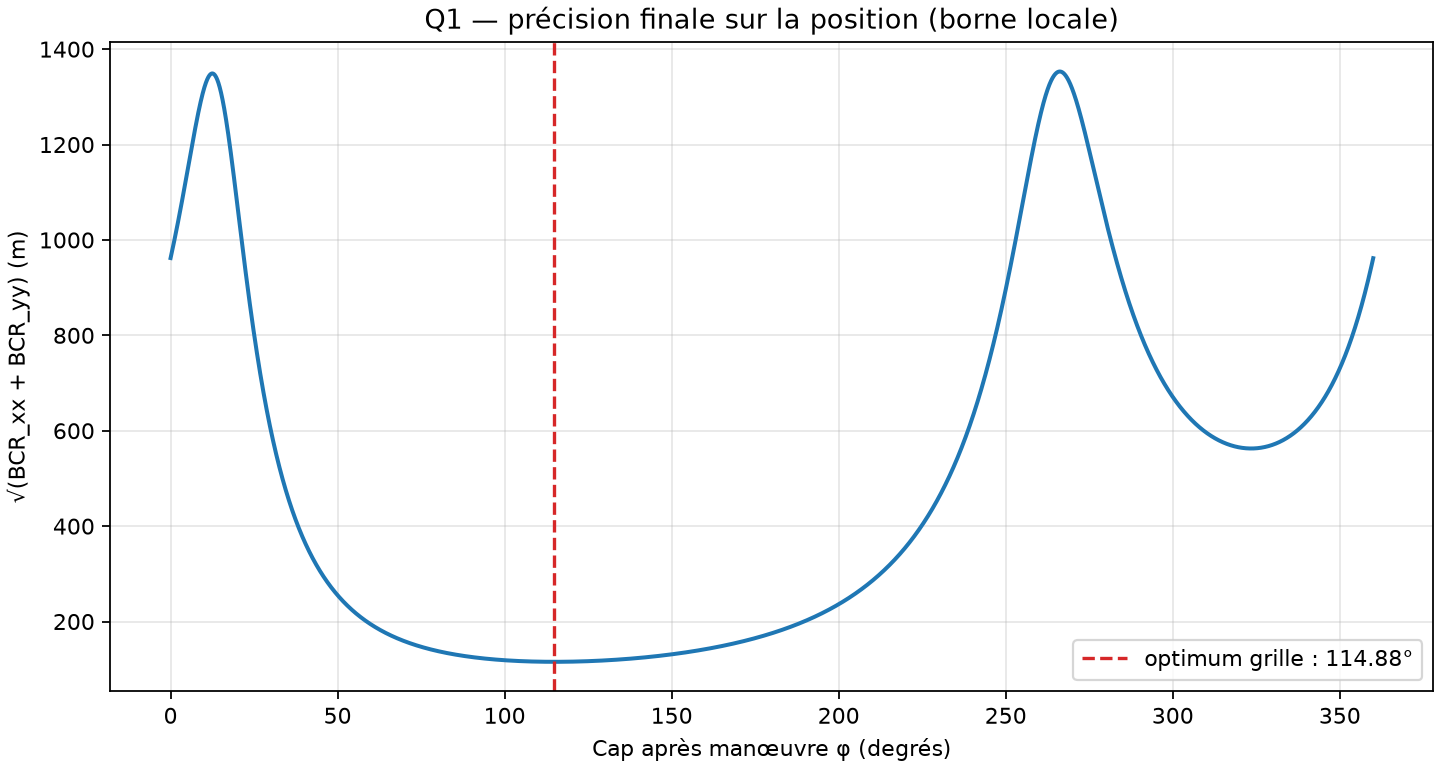
\includegraphics[width=0.65\textwidth]{q1_grille.png}
\caption{RMS finale de position en fonction de l'angle de manœuvre $\varphi$.}
\label{fig:q1_grille}
\end{figure}

La courbe de la figure~\ref{fig:q1_grille} présente un minimum principal autour de $115^\circ$. Une autre zone de minimum apparaît autour de $325^\circ$, mais elle conduit à une incertitude plus importante. Les variations de la courbe montrent que la précision du pistage dépend fortement du cap choisi, c'est-à-dire de la géométrie relative entre l'observateur et la cible.

\begin{figure}[ht]
\centering
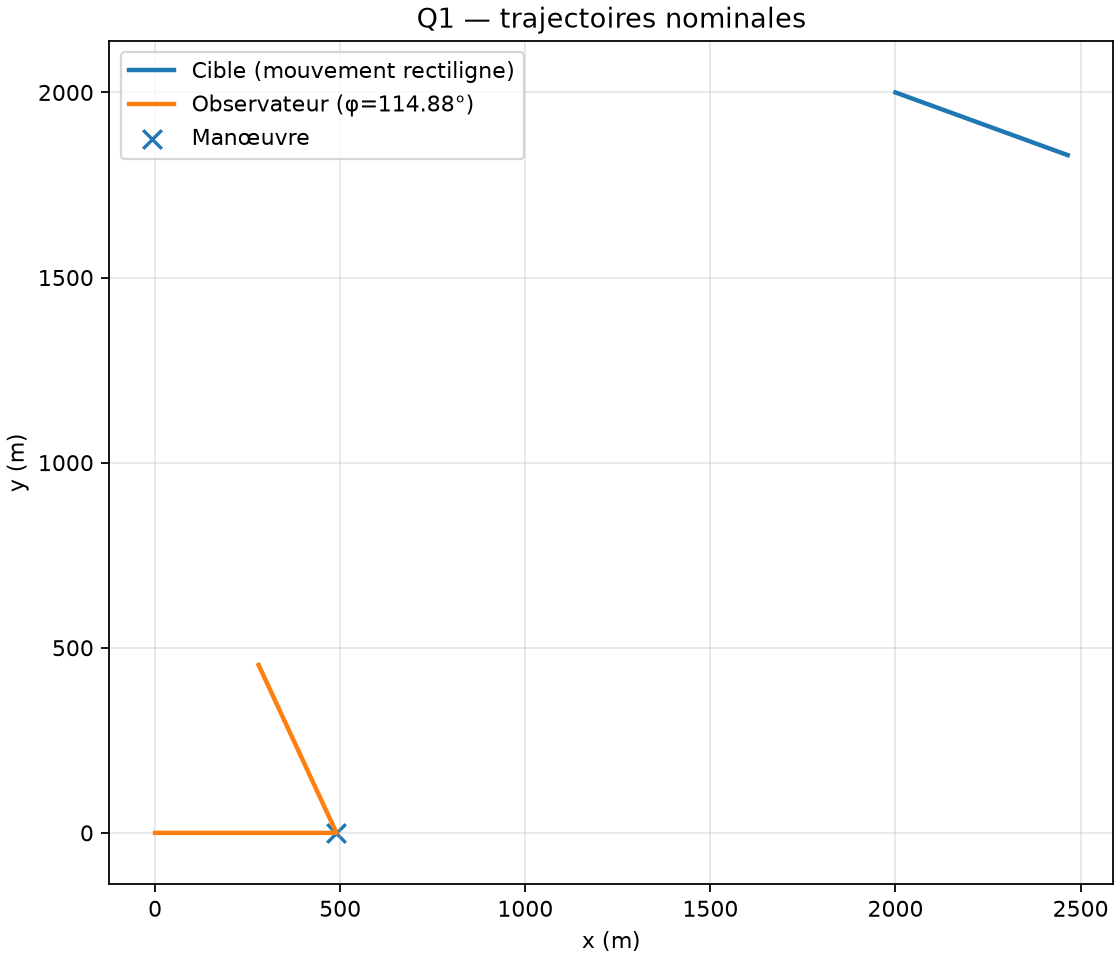
\includegraphics[width=0.5\textwidth]{q1_trajectoires.png}
\caption{Trajectoires nominales de la cible et de l'observateur pour le cap optimal.}
\label{fig:q1_trajectoires}
\end{figure}

La figure~\ref{fig:q1_trajectoires} montre les trajectoires nominales pour l'angle optimal. La cible suit une trajectoire rectiligne à vitesse constante, tandis que l'observateur se déplace selon $+x$, puis change de cap. Ce changement de direction modifie la géométrie d'observation et améliore les conditions de mesure angulaire. Le point de manœuvre est indiqué sur la figure.

\begin{figure}[ht]
\centering
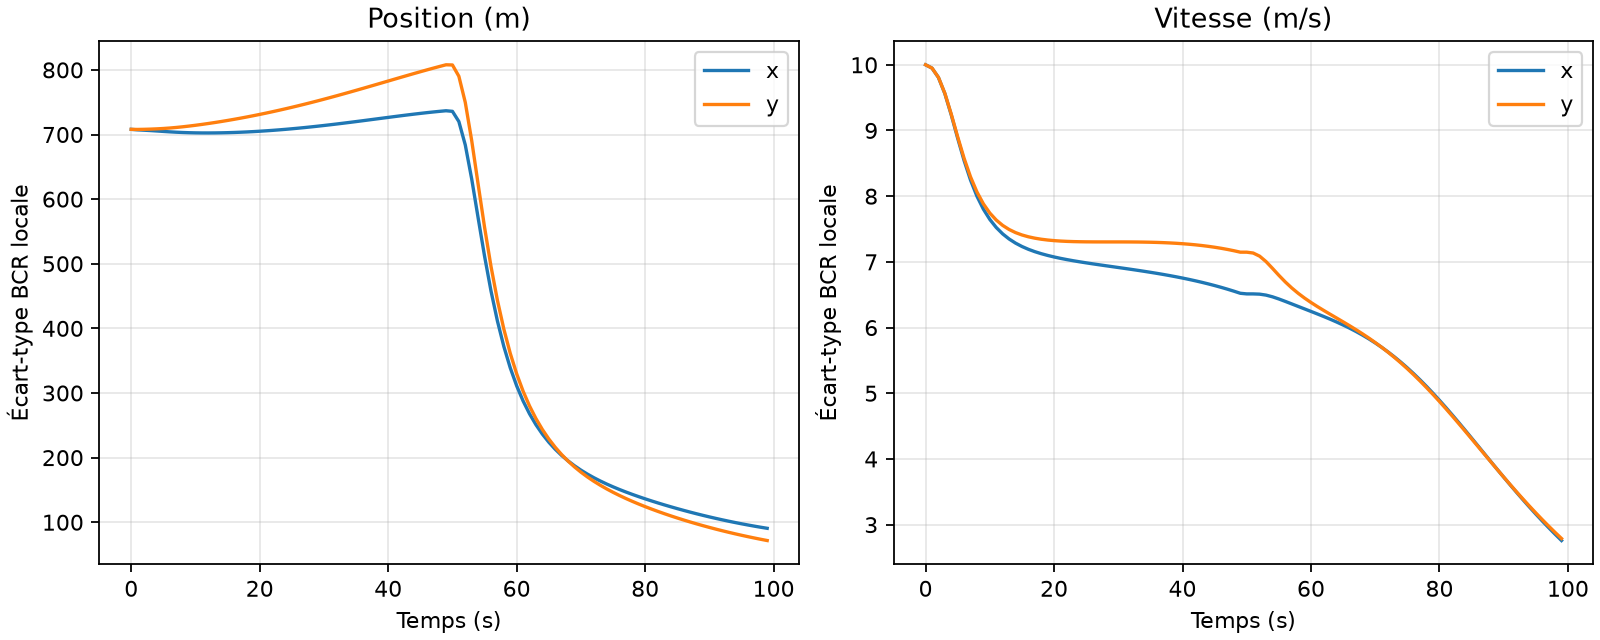
\includegraphics[width=\textwidth]{q1_incertitudes.png}
\caption{Évolution temporelle des écarts-types associés à la BCR locale, pour la position et la vitesse.}
\label{fig:q1_incertitudes}
\end{figure}

La figure~\ref{fig:q1_incertitudes} montre l'évolution des écarts-types associés à la borne. Les incertitudes sur la position augmentent légèrement pendant la première partie de la trajectoire : tant que l'observateur conserve son cap initial, les mesures angulaires déterminent mal la position de la cible. Au voisinage de la manœuvre ($t \approx 50$\,s), les incertitudes diminuent fortement, car le changement de cap apporte une information nouvelle sur l'état. Elles continuent ensuite globalement à diminuer jusqu'à la dernière mesure. Les incertitudes sur la vitesse diminuent également au cours du temps, selon la géométrie d'observation.

\subsection{Bilan de la partie 1}

L'étude du cas $\varphi = 0$ sans information a priori met en évidence une perte d'observabilité : la matrice d'information finale est singulière lorsque l'observateur conserve une trajectoire rectiligne. L'optimisation numérique identifie un angle de manœuvre optimal de $114{,}9^\circ$ pour le scénario étudié, avec une RMS finale minimale de $115{,}540$\,m. La manœuvre de l'observateur joue donc un rôle essentiel dans l'observabilité et la précision du pistage, et la BCR permet de comparer les trajectoires possibles avant toute expérience.

% =====================================================================
\section{Partie 2 --- Dynamique bruitée : BCR et comparaison avec l'EKF}
% =====================================================================

\subsection{Position du problème}

Un objet se déplace en ligne droite. Son état est composé de sa position et de sa vitesse, $X_k = (s_k, v_k)^\top$, avec un modèle à vitesse constante :
\begin{equation}
X_k = \Phi X_{k-1} + \eta_k, \qquad
\Phi = \begin{pmatrix} 1 & \Delta t \\ 0 & 1 \end{pmatrix}, \qquad
\eta_k \sim \N(0, Q), \qquad
Q = \begin{pmatrix} 10^{-4} & 0 \\ 0 & 10^{-2} \end{pmatrix},
\label{eq:dyn}
\end{equation}
avec $\Delta t = 1$\,s et l'a priori $X_0 \sim \N\big((0, 5)^\top, \diag(100, 1)\big)$.
Un capteur placé en $C = (x_c, y_c) = (0, -20)$ mesure uniquement l'azimut (l'angle) de l'objet :
\begin{equation}
z_k = \theta_k + \nu_k, \qquad \theta_k = \atantwo(0 - y_c,\; s_k - x_c), \qquad \nu_k \sim \N\big(0, (1^\circ)^2\big).
\label{eq:mes}
\end{equation}
La mesure est non linéaire et ne dépend que de $s_k$. La vitesse n'est jamais observée directement. On ne peut l'inférer qu'à partir de l'évolution de l'angle au cours du temps.

\subsection{Question 2a : calcul de la BCR avec bruit de dynamique}

\paragraph{Récursion.}
Pour une dynamique linéaire gaussienne et une mesure non linéaire, la matrice d'information de Fisher $J_k$ vérifie la récursion de Tichavský \emph{et al.}~\cite{tichavsky1998} :
\begin{equation}
\boxed{\;
J_{k+1} = \big(\Phi J_k^{-1} \Phi^\top + Q\big)^{-1} + \E_{X_{k+1}}\!\Big[H_{k+1}(X_{k+1})^\top R^{-1} H_{k+1}(X_{k+1})\Big]
\;}
\label{eq:pcrb}
\end{equation}
avec $J_0 = P_0^{-1}$ et $\BCR_k = J_k^{-1}$.
Chaque pas comporte deux parties :
\begin{itemize}[nosep]
  \item \textbf{Prédiction (perte d'information).} $\Phi J_k^{-1} \Phi^\top + Q$ est la borne prédite sur la covariance. Son inverse donne l'information prédite. Plus $Q$ est grand, plus on perd d'information entre deux mesures.
  \item \textbf{Mesure (gain d'information).} La nouvelle mesure d'angle ajoute $H^\top R^{-1} H$, moyenné sur les états vrais possibles.
\end{itemize}
Il s'agit de la forme informationnelle du filtre de Kalman. La seule différence est l'espérance : comme $h$ est non linéaire, $H$ dépend de l'état et doit être moyenné sur la loi de $X_{k+1}$.
Pour $Q = 0$, le premier terme devient $\Phi^{-\top} J_k \Phi^{-1}$, ce qui correspond à la récursion de la partie~1. Le code traite les deux cas de la même façon : il forme $P_{\mathrm{pred}} = \Phi J_k^{-1} \Phi^\top + Q$, puis l'inverse.

\paragraph{Jacobienne de la mesure.}
Pour $\theta = \atantwo(y, x)$, on a $d\theta = (-y\,dx + x\,dy)/(x^2 + y^2)$. Avec $x = s - x_c$ et $y = -y_c$ (constante), on obtient :
\begin{equation}
H(X) = \begin{pmatrix} \dfrac{\partial\theta}{\partial s} & \dfrac{\partial\theta}{\partial v} \end{pmatrix}
= \begin{pmatrix} \dfrac{y_c}{r^2} & 0 \end{pmatrix},
\qquad r^2 = (s - x_c)^2 + y_c^2,
\end{equation}
d'où l'information apportée par une mesure :
\begin{equation}
H^\top R^{-1} H = \frac{y_c^2}{\sigma_\theta^2\, r^4} \begin{pmatrix} 1 & 0 \\ 0 & 0 \end{pmatrix}.
\label{eq:info}
\end{equation}
Elle décroît en $1/r^4$. Comme l'objet avance à environ $5$\,m/s, une mesure d'angle à $t = 30$\,s apporte environ $10^4$ fois moins d'information qu'une mesure à $t = 1$\,s.

\paragraph{Calcul de l'espérance par Monte-Carlo.}
L'espérance dans~\eqref{eq:pcrb} n'a pas de forme explicite. On l'approche avec $M$ échantillons :
\begin{equation}
\E\big[H^\top R^{-1} H\big] \approx \frac1M \sum_{m=1}^{M} H\big(X_{k+1}^{(m)}\big)^\top R^{-1} H\big(X_{k+1}^{(m)}\big).
\end{equation}
Les échantillons sont tirés selon la \emph{loi a priori (non conditionnelle)} de $X_{k+1}$. On tire $X_0^{(m)} \sim \N(\bar X_0, P_0)$, puis on propage chaque échantillon par $X_{k+1}^{(m)} = \Phi X_k^{(m)} + \eta_k^{(m)}$, avec le $Q$ supposé par la borne. Ils ne doivent \emph{pas} être tirés selon la loi a posteriori d'un filtre : la BCR ne dépend que du modèle, et non d'un filtre ou d'un jeu de mesures particulier.
Avec $M = 15\,000$, l'erreur relative de Monte-Carlo est d'environ $1/\sqrt{M} \approx 1\,\%$, ce qui est négligeable.

\paragraph{Vérification à $t = 1$.}
En évaluant $H$ à la position moyenne $s_1 \approx 5$\,m, on obtient $|H| \approx 20/425 = 0{,}047$\,rad/m, soit un écart-type équivalent $\sqrt{R}/|H| \approx 0{,}01745/0{,}047 \approx 0{,}37$\,m.
Ce résultat est proche de la valeur calculée $\sqrt{\BCR_{ss}} = 0{,}42$\,m (tableau~\ref{tab:resultats}). Le petit écart vient du fait que le code moyenne $H$ sur la dispersion de $s_1$ au lieu de l'évaluer en sa moyenne.
En revanche, $\sqrt{\BCR_{vv}}$ reste à $\approx 1$\,m/s, sa valeur a priori, car une seule mesure d'angle ne contient aucune information sur la vitesse.

\subsection{Question 2b : comparaison de la BCR et de l'EKF}

\paragraph{Protocole.}
Le même EKF (mise à jour sous forme de Joseph, avec repliement de l'angle d'innovation) est appliqué à $N = 500$ trajectoires simulées sur $30$\,s. On compare trois cas (tableau~\ref{tab:cas}) ; les cas B et C utilisent exactement les mêmes trajectoires et les mêmes exécutions de l'EKF, seule la borne change.

\begin{table}[ht]
\centering
\caption{Bruit de dynamique supposé dans chaque cas.}
\label{tab:cas}
\begin{tabular}{lcccc}
\toprule
Cas & Vérité & EKF & BCR & Question \\
\midrule
A & $Q = 0$ & $Q = 0$ & $Q = 0$ & Q2b-(1) \\
B & $Q \neq 0$ & $Q \neq 0$ & $Q = 0$ & Q2b-(2) \\
C & $Q \neq 0$ & $Q \neq 0$ & $Q \neq 0$ & Q2b-(3) \\
\bottomrule
\end{tabular}
\end{table}

Pour chaque composante $i \in \{s, v\}$, on trace trois quantités à $3\sigma$ :
\begin{align}
\BCR &: \; 3\sqrt{(J_k^{-1})_{ii}} && \text{(meilleure erreur atteignable)}, \\
\EKF &: \; 3\sqrt{\E\big[P^{\EKF}_{k,ii}\big]} && \text{(erreur annoncée par le filtre)}, \\
\RMSE &: \; 3\sqrt{\E\big[(\hat X_{k,i} - X_{k,i})^2\big]} && \text{(erreur réellement commise)}.
\end{align}
On évalue ainsi deux propriétés :
\begin{itemize}[nosep]
  \item la \textbf{consistance}, $\RMSE \approx \EKF$ : le filtre connaît sa propre précision ;
  \item l'\textbf{efficacité}, $\RMSE \approx \BCR$ : le filtre est proche de l'optimum.
\end{itemize}

\paragraph{Résultats.}

\begin{table}[ht]
\centering
\caption{Écarts-types ($1\sigma$ ; les figures montrent $3\sigma$). Position $s$ en m, vitesse $v$ en m/s. $N = 500$ simulations, $M = 15\,000$.}
\label{tab:resultats}
\begin{tabular}{cr cc cc cc}
\toprule
& & \multicolumn{2}{c}{BCR} & \multicolumn{2}{c}{EKF} & \multicolumn{2}{c}{RMSE} \\
\cmidrule(lr){3-4}\cmidrule(lr){5-6}\cmidrule(lr){7-8}
Cas & $k$ & $s$ & $v$ & $s$ & $v$ & $s$ & $v$ \\
\midrule
A & 1  & 0,42 & 0,99  & 0,37 & 0,99  & 2,08 & 1,05 \\
A & 5  & 0,48 & 0,17  & 0,70 & 0,21  & 1,12 & 0,71 \\
A & 10 & 0,67 & 0,095 & 1,06 & 0,13  & 2,17 & 0,43 \\
A & 30 & 1,68 & 0,063 & 2,56 & 0,093 & 5,58 & 0,25 \\
\midrule
B & 1  & 0,42 & 0,99  & 0,37 & 1,00  & 1,81 & 1,05 \\
B & 5  & 0,48 & 0,17  & 0,68 & 0,25  & 1,07 & 0,64 \\
B & 10 & 0,67 & 0,095 & 1,13 & 0,25  & 1,75 & 0,38 \\
B & 30 & 1,68 & 0,063 & 4,47 & 0,40  & 4,58 & 0,39 \\
\midrule
C & 1  & 0,42 & 1,00  & 0,37 & 1,00  & 1,81 & 1,05 \\
C & 5  & 0,49 & 0,22  & 0,68 & 0,25  & 1,07 & 0,64 \\
C & 10 & 0,79 & 0,23  & 1,13 & 0,25  & 1,75 & 0,38 \\
C & 30 & 3,53 & 0,37  & 4,47 & 0,40  & 4,58 & 0,39 \\
\bottomrule
\end{tabular}
\end{table}

\begin{table}[ht]
\centering
\caption{Rapports à $k = 30$.}
\label{tab:rapports}
\begin{tabular}{lcccc}
\toprule
Cas & $\RMSE/\EKF$ ($s$) & $\RMSE/\EKF$ ($v$) & $\RMSE/\BCR$ ($s$) & $\RMSE/\BCR$ ($v$) \\
\midrule
A & 2,2 & 2,6 & 3,3 & 3,9 \\
B & 1,0 & 1,0 & 2,7 & 6,2 \\
C & 1,0 & 1,0 & 1,3 & 1,04 \\
\bottomrule
\end{tabular}
\end{table}

\paragraph{Cas A : aucun bruit de dynamique (Q2b-1).}

\begin{figure}[ht]
\centering
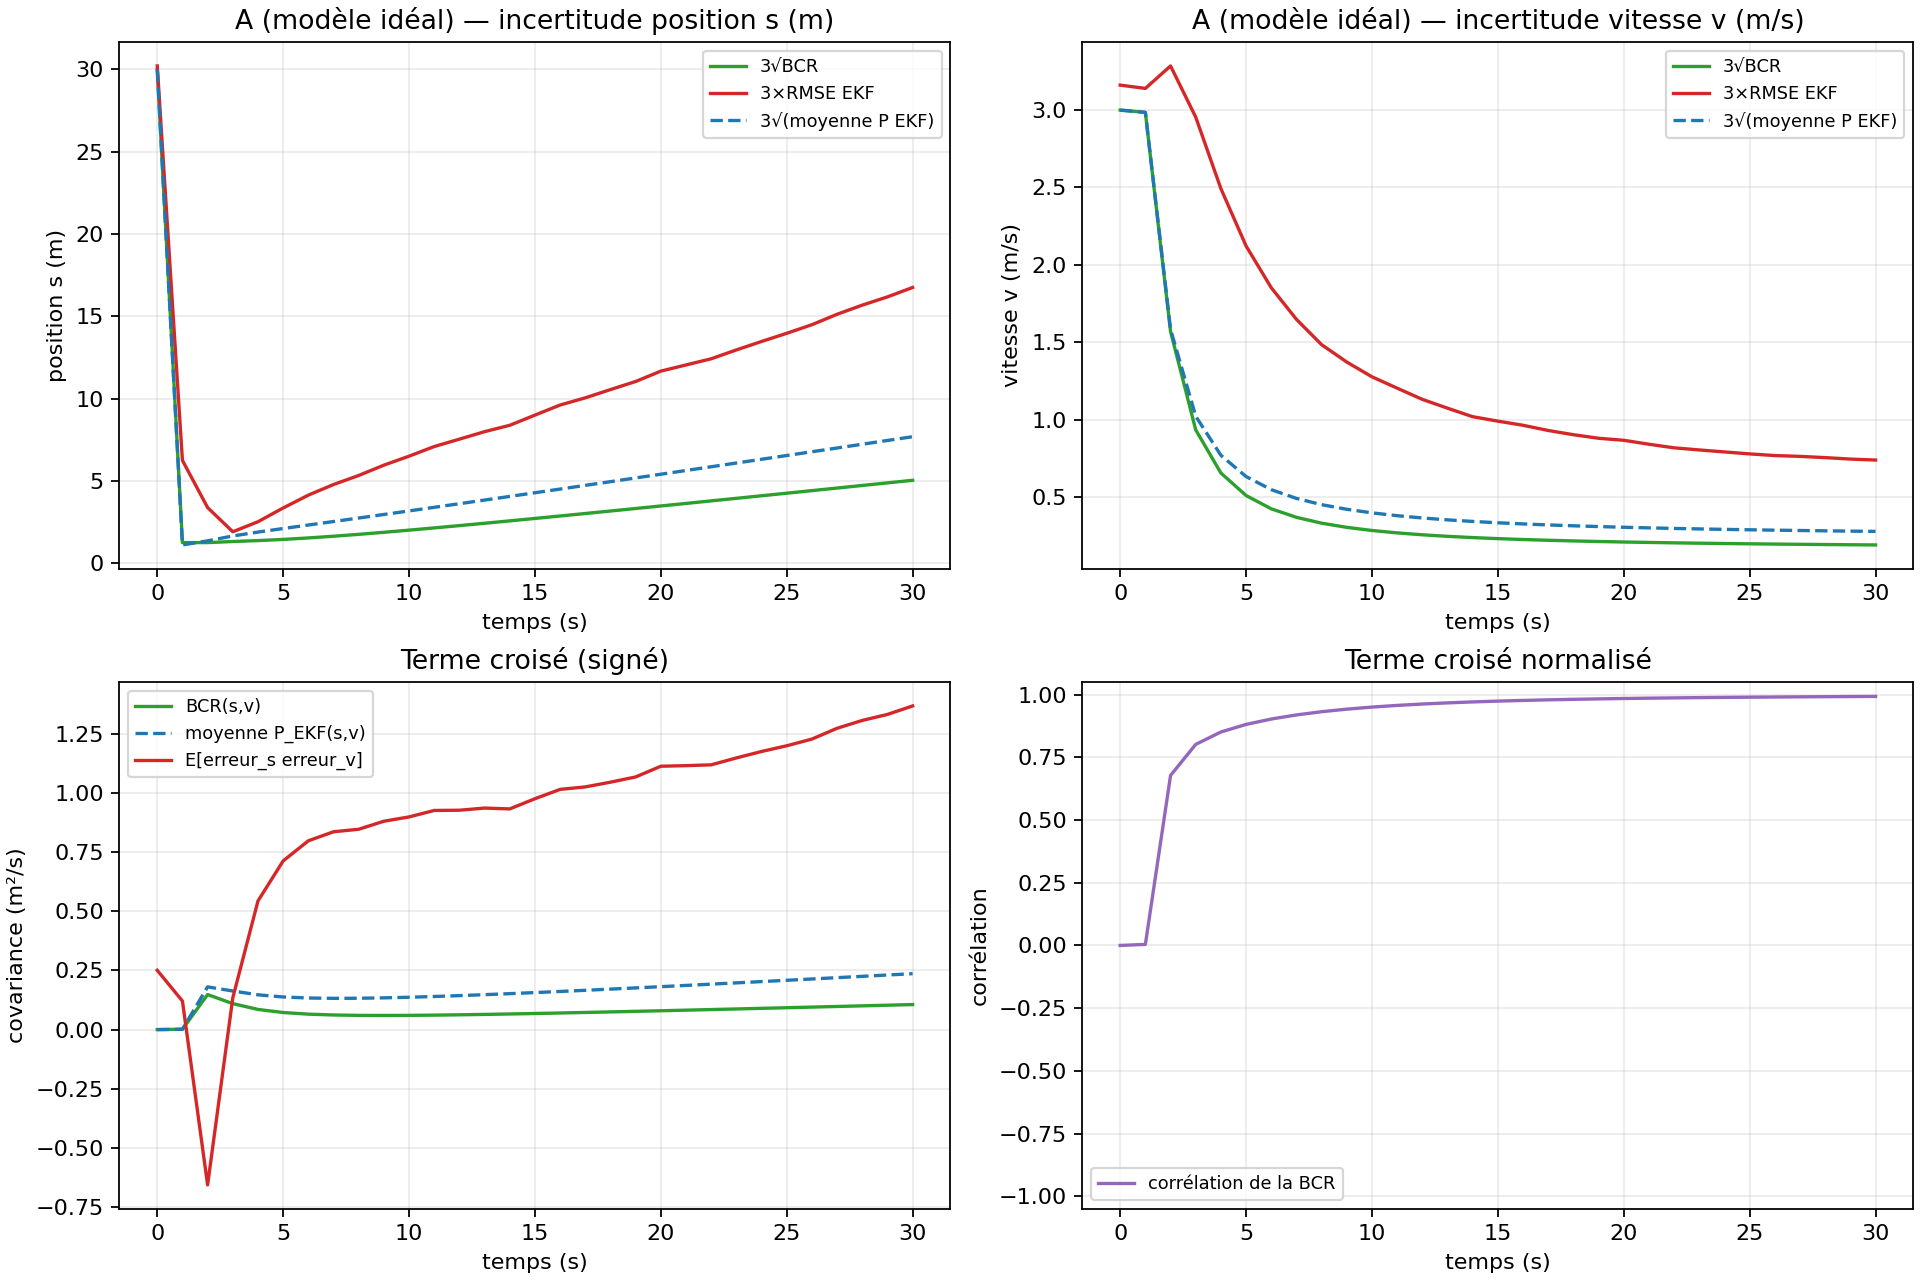
\includegraphics[width=\linewidth]{experience_A.png}
\caption{Cas A : $Q = 0$ pour la vérité, l'EKF et la BCR.}
\label{fig:A}
\end{figure}

La BCR se comporte comme attendu pour une dynamique déterministe (figure~\ref{fig:A}). La borne sur la position descend d'abord à $0{,}4$\,m, tant que l'objet est proche du capteur, puis augmente lentement car les mesures d'angle apportent de moins en moins d'information~\eqref{eq:info}. La borne sur la vitesse continue de diminuer : chaque nouvelle mesure affine l'estimation de la vitesse, qui est constante.

L'EKF, en revanche, \textbf{n'est pas consistant}. Son erreur réelle est 2 à 3 fois plus grande que la covariance qu'il annonce, et elle est loin de la borne (facteur $3{,}3$ en position et $3{,}9$ en vitesse à $k = 30$). Deux mécanismes l'expliquent :
\begin{enumerate}[nosep]
  \item \emph{Erreur de linéarisation à la première mise à jour.} L'incertitude initiale sur la position ($\sigma = 10$\,m) est du même ordre que la distance au capteur ($20$\,m). Sur un tel intervalle, $\atantwo$ est fortement non linéaire : la jacobienne $H(\hat X^-)$ est une mauvaise approximation, et la première correction est biaisée. On le voit à $k = 1$ : RMSE de $2{,}1$\,m contre une borne de $0{,}4$\,m.
  \item \emph{Aucun mécanisme de rattrapage.} Avec $Q = 0$, $P_k$ ne fait que décroître, donc le gain $K_k \to 0$. Le filtre accorde de moins en moins de poids aux nouvelles mesures. L'erreur initiale est propagée par la dynamique, et $e_s \approx e_s^{(0)} + t\, e_v$ croît linéairement avec le temps.
\end{enumerate}

\paragraph{Cas B : bruit de dynamique dans la vérité et l'EKF, pas dans la BCR (Q2b-2).}

\begin{figure}[ht]
\centering
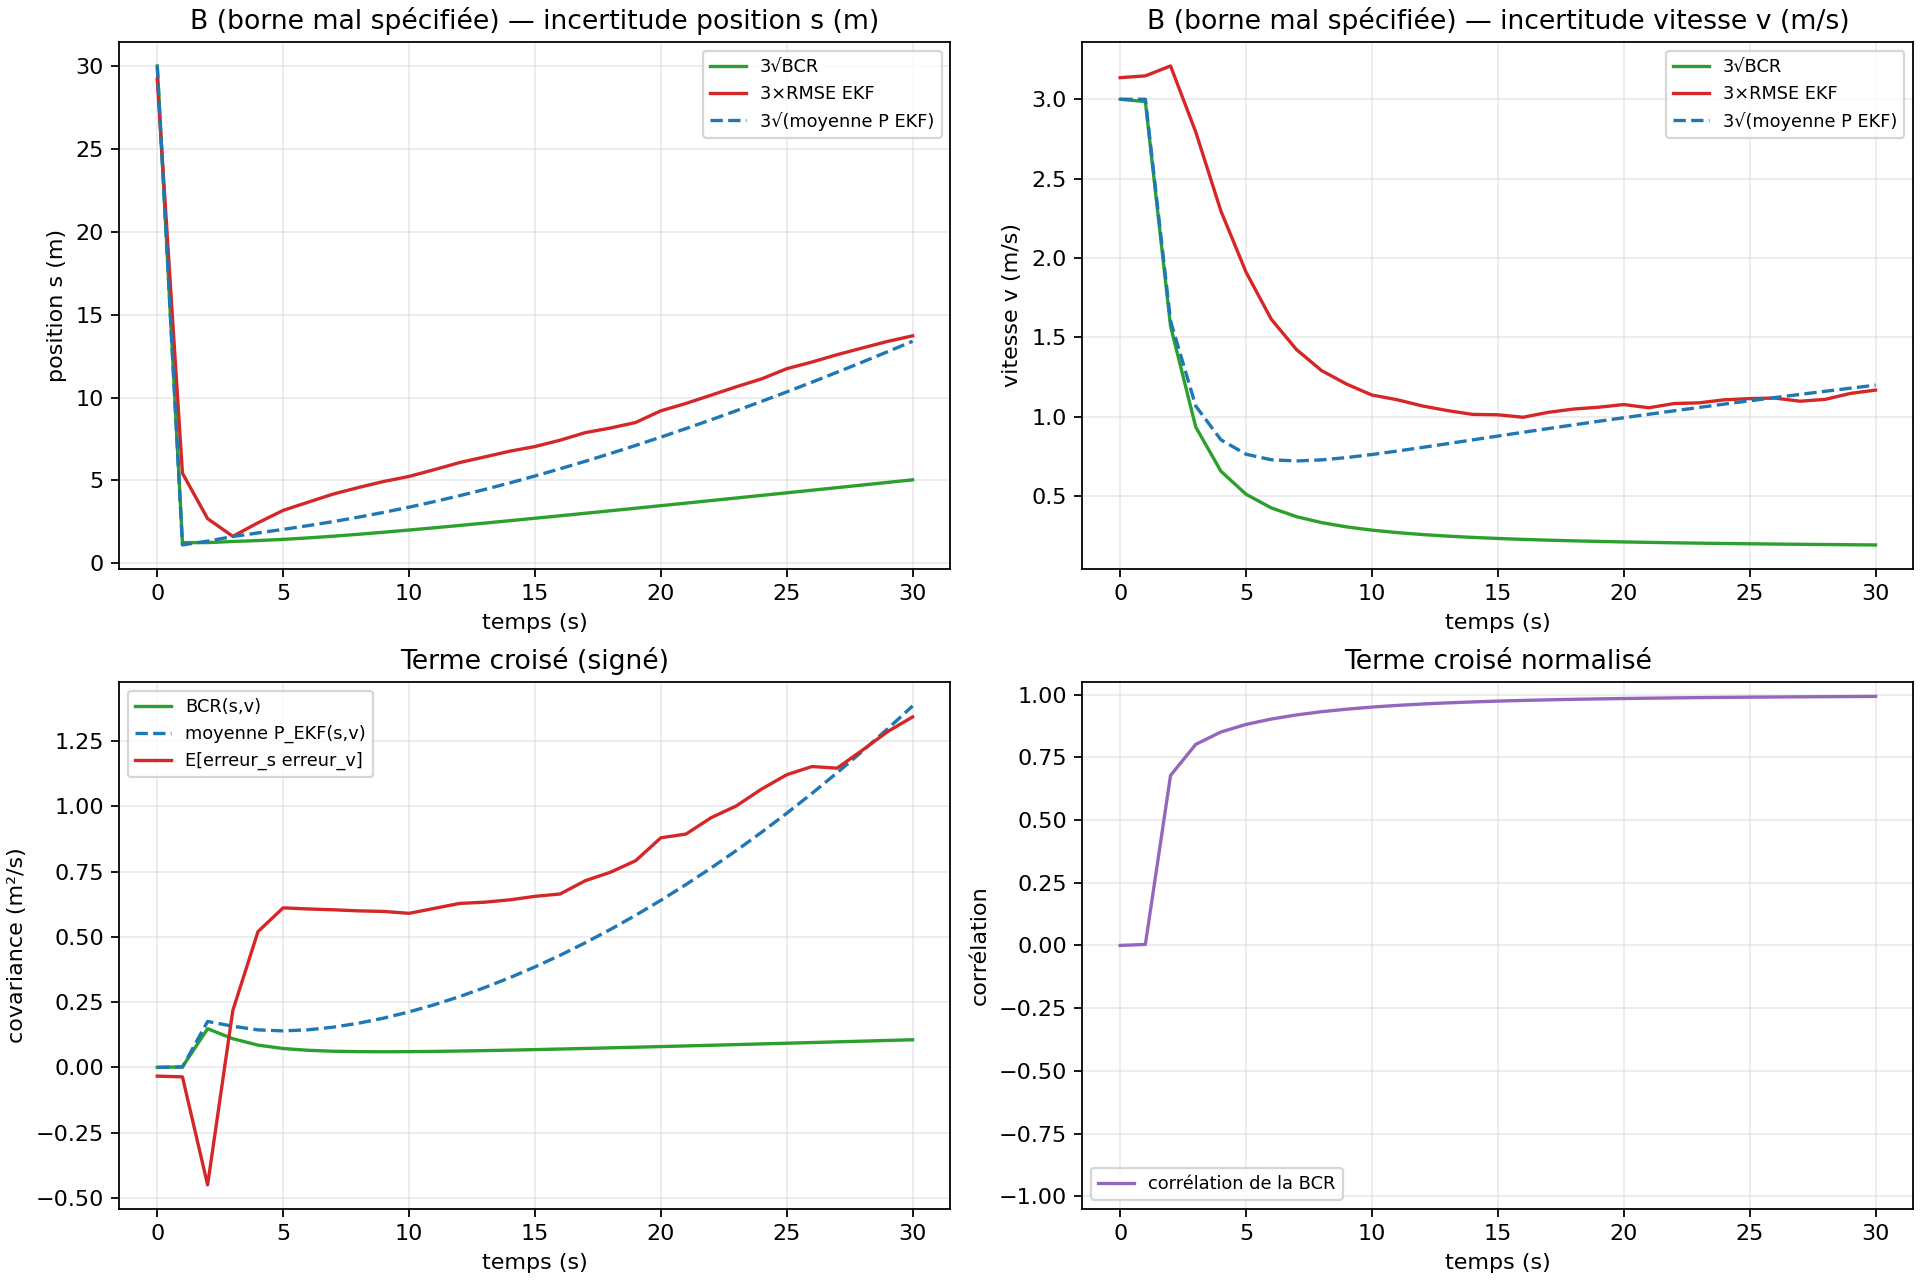
\includegraphics[width=\linewidth]{experience_B.png}
\caption{Cas B : $Q \neq 0$ pour la vérité et l'EKF, $Q = 0$ pour la BCR.}
\label{fig:B}
\end{figure}

L'EKF est maintenant \textbf{consistant} : $\RMSE \approx \EKF$ pour les deux composantes ($4{,}58$ contre $4{,}47$\,m et $0{,}39$ contre $0{,}40$\,m/s à $k = 30$, figure~\ref{fig:B}). Avec $Q > 0$, la covariance prédite ne tend pas vers zéro. Le gain reste donc significatif et le filtre continue de se corriger grâce aux nouvelles mesures : l'erreur de linéarisation initiale est oubliée.

La borne, elle, est \textbf{mal spécifiée}. C'est la même courbe que dans le cas A, car elle ignore le bruit de dynamique. Elle est $2{,}7$ fois plus basse que la RMSE en position et $6{,}2$ fois plus basse en vitesse.
Cette courbe n'est pas une borne valide pour ce problème : l'inégalité de Cramér-Rao n'est vraie que pour le modèle utilisé pour calculer $J_k$. Elle indique seulement ce qui serait possible \emph{si} l'objet ne subissait aucune accélération aléatoire. Il serait donc faux d'en conclure que l'EKF est loin de l'optimum.

\paragraph{Cas C : même bruit de dynamique partout (Q2b-3).}

\begin{figure}[ht]
\centering
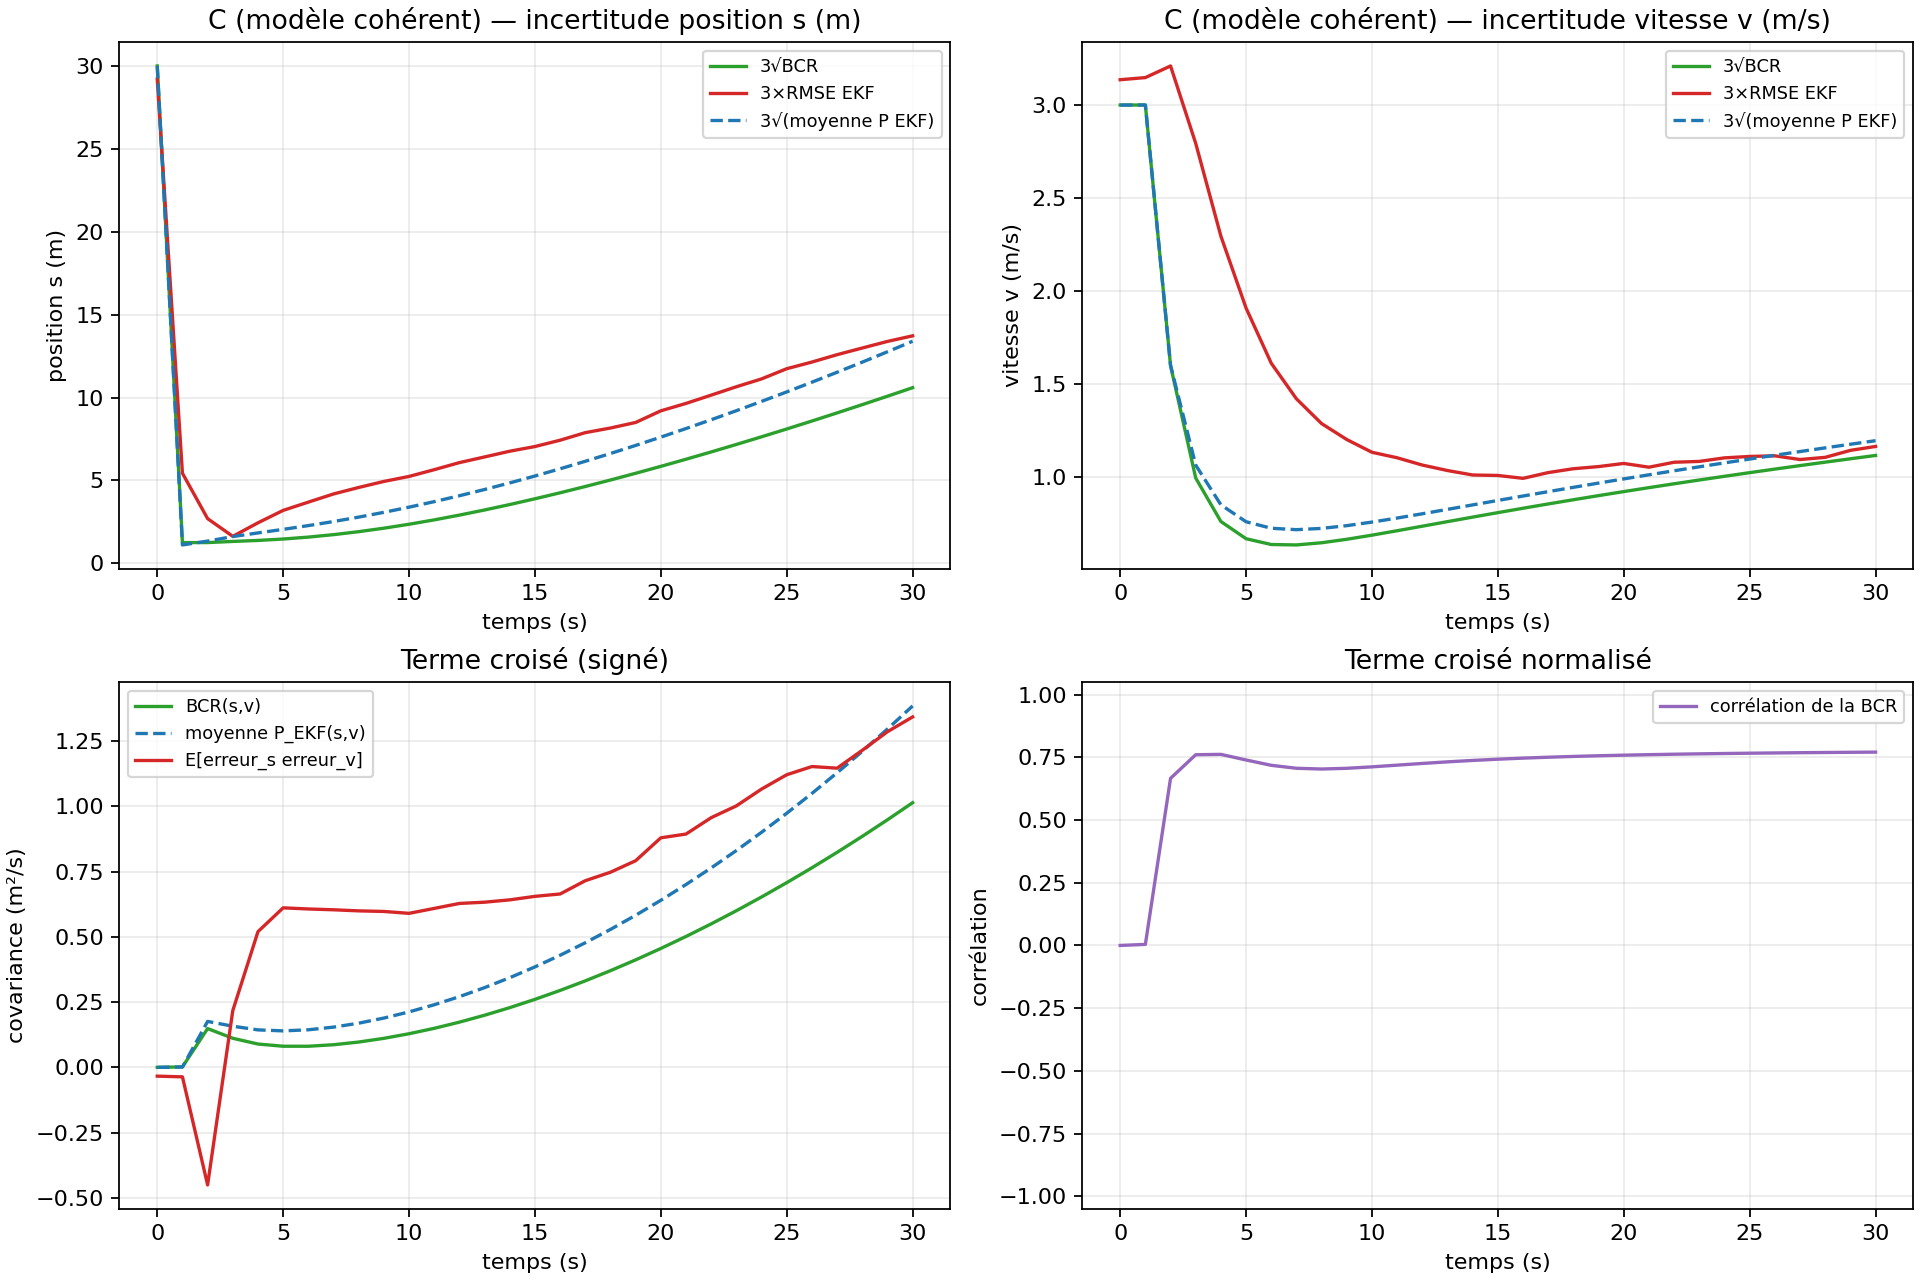
\includegraphics[width=\linewidth]{experience_C.png}
\caption{Cas C : même $Q \neq 0$ pour la vérité, l'EKF et la BCR.}
\label{fig:C}
\end{figure}

Les trois courbes sont dans l'ordre attendu : $\BCR \le \RMSE \approx \EKF$ (figure~\ref{fig:C}).
La borne augmente maintenant avec le temps pour les deux composantes : chaque pas ajoute l'incertitude $Q$, tandis que l'information apportée par les mesures décroît en $1/r^4$. Le bruit de dynamique finit par dominer.
L'EKF est \textbf{proche de l'efficacité} : à $k = 30$, sa RMSE dépasse la borne de $4\,\%$ en vitesse et de $30\,\%$ en position. L'écart plus important au début ($t < 15$\,s) correspond au coût des premières mises à jour non linéaires. La borne ne paie pas ce coût, car elle évalue $H$ aux états vrais.

\begin{remarque}
À $k = 1$, l'EKF annonce $0{,}37$\,m, légèrement \emph{en dessous} de la BCR ($0{,}42$\,m). Cela ne contredit pas la théorie : la borne s'applique à l'erreur réelle (RMSE $= 1{,}81$\,m), et non à la covariance calculée par le filtre, qui n'est qu'une approximation.
\end{remarque}

\paragraph{Comparaison des cas B et C.}

\begin{figure}[ht]
\centering
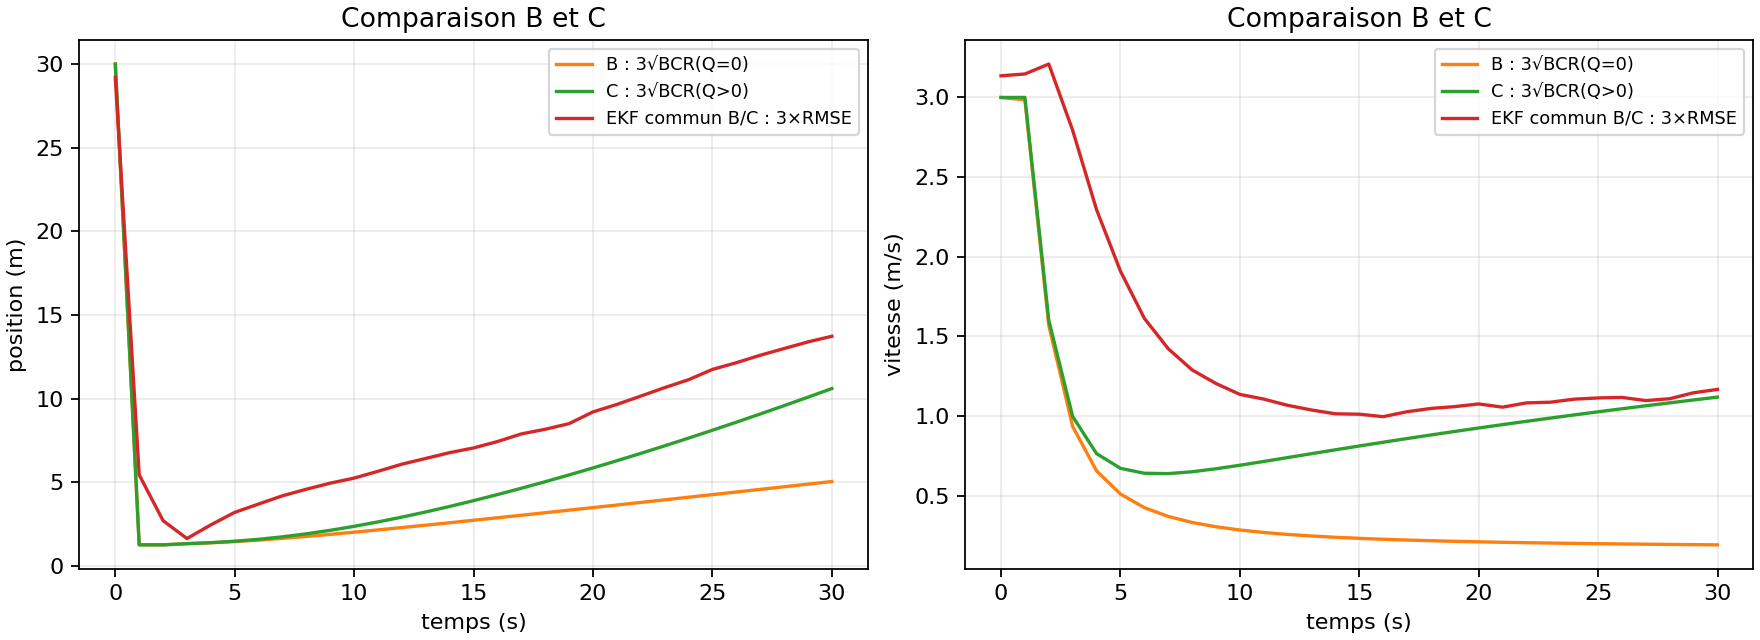
\includegraphics[width=\linewidth]{comparison_B_C.png}
\caption{Comparaison des bornes B ($Q = 0$) et C ($Q \neq 0$) avec la RMSE de l'EKF commun.}
\label{fig:BC}
\end{figure}

Les deux bornes coïncident pendant les $5$ premières secondes environ : les mesures sont alors très informatives et peu de bruit de dynamique s'est accumulé (figure~\ref{fig:BC}). Elles divergent ensuite : à $k = 30$, la borne correcte (C) est $2{,}1$ fois plus grande en position et $5{,}9$ fois plus grande en vitesse que la borne mal spécifiée (B).
\textbf{Ignorer $Q$ dans la borne surestime fortement la performance atteignable}, en particulier pour la vitesse, qui est la composante directement soumise au bruit.

\subsection{Bilan de la partie 2}

\begin{itemize}[nosep]
  \item \textbf{Q2a.} La BCR avec bruit de dynamique se calcule récursivement à partir du seul modèle $(P_0, \Phi, Q, h, R)$. Une moyenne de Monte-Carlo permet de traiter la mesure non linéaire. Comme elle ne nécessite aucune donnée de mesure, elle peut être calculée avant toute expérience, par exemple pour dimensionner un système.
  \item \textbf{Q2b.} La comparaison RMSE/EKF teste la consistance du filtre : il est non consistant en A, et consistant en B et C. La comparaison RMSE/BCR teste son efficacité, et n'a de sens que si la borne utilise le vrai modèle (cas C). Dans ce cas, l'EKF est proche de l'efficacité une fois le régime transitoire passé.
  \item Un peu de bruit de dynamique dans le filtre le rend plus robuste : le gain reste ouvert et le filtre peut se remettre des erreurs de linéarisation.
\end{itemize}

\begin{remarque}[Limite]
La BCR est une borne locale, fondée sur la courbure de la vraisemblance. Elle peut être optimiste lorsque la loi a posteriori est étalée ou multimodale, ce qui est le cas ici au premier instant. Des bornes globales, comme celle de Ziv-Zakai, sont plus adaptées à ce régime.
\end{remarque}

% =====================================================================
\section*{Conclusion}
% =====================================================================

Ce TP a montré que la borne de Cramér-Rao est un outil simple et puissant pour évaluer, \emph{a priori} et à partir du seul modèle, la meilleure précision atteignable par un estimateur.
Sa formulation récursive s'adapte naturellement au filtrage et permet d'optimiser un système, par exemple la manœuvre d'un observateur, avant toute expérience.
La comparaison avec un filtre de Kalman étendu permet de distinguer deux questions : la consistance du filtre et son efficacité.
Elle rappelle aussi que la borne n'a de sens que si elle repose sur le vrai modèle, et qu'elle reste une borne locale, à compléter par des bornes globales en faible rapport signal sur bruit.

\begin{thebibliography}{9}
\bibitem{tichavsky1998}
P.~Tichavský, C.~H. Muravchik et A.~Nehorai,
\newblock « Posterior Cramér-Rao bounds for discrete-time nonlinear filtering »,
\newblock \emph{IEEE Transactions on Signal Processing}, vol.~46, n\textsuperscript{o}~5, p.~1386--1396, 1998.
\bibitem{dambreville}
F.~Dambreville,
\newblock \emph{Filtrage bayésien et approximation particulaire --- Bornes de Cramér-Rao}, support de cours, ONERA / ENSTA, 2026.
\end{thebibliography}

\end{document}
